%!TEX root = ../thesis.tex
%*******************************************************************************
%*********************************** Statistics *********
%*******************************************************************************


\chapter{Statistical data analysis}\label{ch:statistics}

\ifpdf
    \graphicspath{{chapter-statistics/Figs/Raster/}{chapter-statistics/Figs/PDF/}{chapter-statistics/Figs/}}
\else
    \graphicspath{{chapter-statistics/Figs/Vector/}{chapter-statistics/Figs/}}
\fi

\glsreset{pdf}

Statistical models are used in order to order to quantify the correspondence between theoretical predictions and the experimental observations in searches for \gls{susy}. This chapter introduces the statistical concepts, methods and formulae used in this work for statistical inference. A frequentist approach to statistics is employed, interpreting probabilities as the frequencies of the outcomes of repeatable experiments that may either be real, based on computer simulations, or mathematical abstraction~\cite{pdg2020,Cranmer:2015nia}. The ensuing description largely follows~\cite{Cranmer:2015nia, Cowan:2010js}

\section{The likelihood function}\label{sec:likelihood_function}
 
In measurements in high energy physics, a \textit{statistical model} $f(\boldsymbol{x}\vert\boldsymbol{\phi})$ is a parametric family of \glspl{pdf} describing the probability of observing data $\boldsymbol{x}$ given a set of model parameters $\phi$ that typically describe parameters of the physical theory or unknown detector effects. The \textit{likelihood function} $L(\boldsymbol{\phi})$ is then numerically equivalent to $f(\boldsymbol{x}\vert\boldsymbol{\phi})$ with $\boldsymbol{x}$ fixed. As opposed to the \gls{pdf} $f(\boldsymbol{x})$ which describes the value of $f$ as a function of $\boldsymbol{x}$ given a fixed set of parameters $\boldsymbol{\phi}$, the likelihood refers to the value of $f$ as a function of $\boldsymbol{\phi}$ given a fixed value of $\boldsymbol{x}$.

Searches for \gls{bsm} physics are typically centred around the measurement of several disjoint binned distributions (called \textit{channels} $c$) that are each associated with different event selection criteria (as opposed to different scattering processes) yielding observed event counts $\boldsymbol{n}$. In such counting experiments where each event is independently drawn from the same underlying distribution, each bin is fundamentally described by a Poisson term. The Poisson probability to observe $n$ events with a expectation of $\nu$ events, is given by
\begin{equation}
	\mathrm{Pois}(n\vert\nu) = \frac{\nu^n}{n!}e^{-\nu}.
\end{equation}
The expectation $\nu_{cb}$ in each channel $c$ and bin $b$ is a sum over the set of physics processes considered (called \textit{samples}). The sample-wise rates are in general a function of the the model parameters $\boldsymbol{\phi}$, that can either be \textit{free parameters} $\boldsymbol{\eta}$ or \textit{constrained parameters} $\boldsymbol{\chi}$. Free parameters directly determined by the Poisson terms for the data observations are called \textit{normalisation factors}. The constrained parameters represent the systematic uncertainties considered in the model. The degree to which they cause a deviation of the expected event rates from the nominal event rates is limited through \textit{constraint terms} $c_{\boldsymbol{\chi}}(a_{\boldsymbol{\chi}}\vert\boldsymbol{\chi})$ that can be viewed as \textit{auxiliary measurements} with global observed data $\boldsymbol{a}$. 

For a given observation $\boldsymbol{x} = (\boldsymbol{n},\boldsymbol{a})$ of observed events $\boldsymbol{n}$ and auxiliary data $\boldsymbol{a}$, the likelihood then reads
\begin{equation}
	L (\boldsymbol{\eta}, \boldsymbol{\chi}) = \prod_{c\in\mathrm{channels}} \prod_{b\in\mathrm{bins_c}} \mathrm{Pois}(n_{cb}\vert\nu_{cb}(\boldsymbol{\eta},\boldsymbol{\chi})) \prod_{\chi\in\boldsymbol{\chi}}c_\chi (a_\chi\vert\chi),
\end{equation}
where, given a certain integrated luminosity, $n_{cb}$ and $\nu_{cb}$ refer to the corresponding observed and expected rate of events, respectively~\cite{ATL-PHYS-PUB-2019-029}. Most of the systematic uncertainties are so-called \textit{interpolation parameters} $\boldsymbol{\alpha}$ representing either normalisation uncertainties or correlated shape uncertainties\improvement{Explain this further}. Their constraint terms $c_{\boldsymbol{\alpha}}(a_{\boldsymbol{\alpha}}\vert\boldsymbol{\alpha})$ are parametrised by a Gaussian with mean $a = 0\vert\alpha$ and variance $\sigma = 1$, with $\alpha = 0$ representing the nominal value. The \textit{up} and \textit{down} variations are then given by $\alpha=\pm 1$, thus representing $\pm 1\sigma$ variations. The impact of any given value of the parameter on the event rates is then evaluated through polynomial interpolation and exponential extrapolation, a method that avoids discontinuous first and second derivatives at $\alpha = 0$ and ensures positive values for the predicted event rates~\cite{Cranmer:1456844}.

Sample rates derived from theory calculations (\ie \gls{mc} simulation), are scaled to the integrated luminosity corresponding to the observed data. The integrated luminosity is itself a measurement that is subject to uncertainties. Therefore, an additional constraint term in the likelihood is needed. It is parametrised by a Gaussian with mean corresponding to the nominal integrated luminosity measurement and variance equal to the integrated luminosity measurement uncertainty.

Uncertainties arising from the finite size of the \gls{mc} datasets often used to derive estimated event rates are modelled by bin-wise scale factors $\gamma_b$. The constraint terms are Gaussian distributions with central value equal to unity and variances calculated from the individual uncertainties of the samples defined in the respective channel.

As the event rate in a given bin can depend on multiple parameters, and, likewise, a single parameter can affect the expected event rate in multiple bins, correlations between the model parameters $\boldsymbol{\phi}$ can occur.

The above prescription for building binned likelihoods is called the \textsc{HistFactory} template~\cite{Cranmer:1456844}. In this work, two independent implementations of the \textsc{HistFactory} template are used. The first implementation uses \textsc{RooFit} and \textsc{RooStats} for fitting (using \texttt{Minuit}), and \textsc{HistFitter}~\cite{HistFitter:2014wma} as interface for steering fits and hypothesis tests and bookkeeping of results. The second implementation uses \texttt{pyhf}, a pure-\texttt{python} implementation of \textsc{HistFactory} that is independent from \textsc{ROOT} and uses computational graph libraries like \texttt{PyTorch}, \textsc{TensorFlow} and \textsc{JAX} to speed up the minimisation process.
 
%\begin{equation}
%	\nu_{cb}(\boldsymbol{\phi}) = \sum_{s\in\mathrm{samples}}{}\nu_{scb}(\boldsymbol{\phi}) = \sum_{s\in\mathrm{samples}}{\left(\prod_{\kappa\in\boldsymbol{\kappa}}\kappa_{scb}(\boldsymbol{\phi})\right)\left(\nu^0_{scb}(\boldsymbol{\phi})+\sum_{\Delta\in\boldsymbol{\Delta}}\Delta_{scb}(\boldsymbol{\phi})\right)},
%\end{equation} 
%where $\nu_{scb}$ are sample-wise event rates determined from \textit{nominal rates} $\nu^0_{scb}$ and a set of multiplicative and additive \textit{rate modifiers} $\boldsymbol{\kappa(\phi)}$ and $\boldsymbol{\Delta(\phi)}$, that are functions of the model parameters (typically only a single parameter per modifier). The modifiers are paired with a constraint term in order to implement systematic uncertainties into the statistical model. The event rates in a given bin can be affected by multiple parameters and single parameters can 

Apart from separating the model parameter set into free and constrained parameters $\boldsymbol{\phi} = (\boldsymbol{\eta},\boldsymbol{\chi})$, a separate partition $\boldsymbol{\phi} = (\boldsymbol{\psi},\boldsymbol{\theta})$ is frequently used in the context of hypothesis testing. Here, $\boldsymbol{\eta}$ are so-called \textit{parameters of interests} of the model for which hypothesis tests are performed, and $\boldsymbol{\theta}$ are \textit{nuisance parameters} that are not of immediate interest but need to be accounted for to correctly model the data. In the search presented in this work, the only \gls{poi} is the \textit{signal strength} parameter $\mu$, representing the ratio of the signal process cross section to its reference cross section as expected from theory. The expectation $\nu_i$ in each bin $i$ can be parametrised through
\begin{equation}
	\nu_b = \mu S_b + B_b,
\end{equation}
where $S_b$ and $B_b$ are the bin-wise expected signal and background rates, respectively. Fixing $\mu = 0$ thus yields an expected event rate containing only \gls{sm} processes (thus called \textit{background-only}), while $\mu = 1$ represents a \textit{signal-plus-background} description at nominal signal cross section. Scanning multiple values of $\mu$ allows to set limits on the visible cross sections of the signal models considered in the search. 
  
\section{Parameter estimation}

Given a likelihood $L(\mu,\boldsymbol{\phi})$ for a fixed set of observations $\boldsymbol{x}$, a measurement can be understood as a parameter estimation. In general, an estimator $\hat{\phi}$ is a function of the observed data used to estimate the true value of the model parameter $\phi$.

In particle physics, the most commonly used estimator is the \gls{mle}. The \glspl{mle} for the model parameters $\boldsymbol{\hat{\phi}}$ are defined to be the parameter values that maximise $L(\boldsymbol{\phi})$, or, equivalently maximise $\ln{L(\boldsymbol{\phi})}$ and minimises $-\ln{L(\boldsymbol{\phi})}$. The logarithm of the likelihood is used for computational reasons, as it not only reduces the computational complexity by avoiding exponentials and products, but also avoids avoids problems of running out of floating point precision. As the logarithm is a monotonically increasing function, $\ln{L(\boldsymbol{\phi})}$ has maxima at the same parameter values as ${L(\boldsymbol{\phi})}$.

The \gls{mle} $\boldsymbol{\hat{\phi}}$ can thus be found by solving
\begin{equation}
 \frac{\partial \ln L}{\partial\phi_i} = 0,
\end{equation}
where the index $i$ runs over all parameters. The solution typically needs to be found numerically using minimisation algorithms. In the following, the parameter estimation is referred to as a \textit{fit} of the model to data, and the maximum likelihood estimates of the parameters are consequently called \textit{best-fit values}.

\section{Statistical tests}

In addition to estimating the values of model parameters, searches for \gls{susy} are naturally interested in claiming discovery (or alternatively exclusion) of hypothesised signal models. In the frequentist approach, this can be formulated in terms of hypothesis tests, evaluating a \textit{null hypothesis} $H_0$ against an \textit{alternative hypothesis} $H_1$, with the goal of rejecting the null hypothesis. For discovering a new signal process, $H_0$ is defined to describe only known \gls{sm} processes (called \textit{background-only} hypothesis), while $H_1$ describes both \gls{sm} background processes as well as the signal process (called \textit{signal plus background hypothesis}). When excluding a signal model the signal plus background hypothesis takes over the role of $H_0$ and is tested against the background-only hypothesis.

The degree of agreement of observed data with a certain hypothesis $H$ is quantified by computing a $p$-value, representing the probability of finding data of greater or more extreme incompatibility under assumption of $H$. The hypothesis can then be considered as excluded if its observed $p$-value is below a specified threshold. It is common to convert the $p$-value into a \textit{significance} $Z$, defined in such a way that a Gaussian distributed observable with measured value $Z$ standard deviations above its mean gives a one-sided upper tail probability equal to $p$. This yields the expression
\begin{equation}
	Z = \Phi^{-1}(1-p),
	\label{eq:significance}
\end{equation}
where $\Phi^{-1}$ is the quantile of the standard Gaussian. Discovery of a signal then conventionally requires a significance of at least $Z = 5$, while exclusion of a signal hypothesis at 95\% confidence level requires a $p$-value of 0.05, \ie $Z = 1.64$~\cite{Cowan:2010js}. 

The $p$-values are calculated using a \textit{test statistic} that parameterises the compatibility between the hypothesis and data in a single value. At the LHC experiments, the test statistics used for hypothesis testing are based on the \textit{profile likelihood ratio}
\begin{equation}
	\lambda(\mu) = \frac{L(\mu,\boldsymbol{\hat{\hat{\theta}}}(\mu))}{L(\hat{\mu},\hat{\boldsymbol{\theta}})},
\end{equation}
where the \textit{conditional maximum likelihood estimates} $\boldsymbol{\hat{\hat{\theta}}}$ are the values of $\boldsymbol{\theta}$ that maximise the likelihood with $\mu$ fixed. The profile likelihood ratio depends explicitly on $\mu$, and implicitly on $\boldsymbol{x} = (\boldsymbol{n},\boldsymbol{a})$, but is asymptotically  (\ie in the limit of a large number of events)independent of the nuisance parameters $\boldsymbol{\theta}$\footnote{Eliminated by choosing specific values of the nuisance parameters for a given $\boldsymbol{x}$ and $\mu$, often referred to as \textit{profiling}.}. The asymptotic independence from $\boldsymbol{\theta}$ follows from Wald's and Wilks' theorems~\cite{wald10.2307/1990256,wilks1938} and is one of the main motivations for using the profile likelihood ratio, as it avoids the problem of having to compute $p$-values for all possible values of $\boldsymbol{theta}$. The profile likelihood ratio takes values between 0 and 1, with $\lambda(\mu) = 1$ corresponding to cases where the tested value of $\mu$ is in good agreement with the observed data.

As the rate of signal processes considered in this work is non-negative, an estimator for $\mu$ must satisfy $\hat{\mu}\geq 0$. In order to avoid the formal complications of having a boundary at $\mu = 0$, it is convenient to consider an effective estimator $\hat{\mu}$ that is allowed to become negative, provided that the respective Poisson terms for $\mu S_b + B_b$ remain positive. By imposing the constraint $\mu \geq 0$ on the test statistic itself, it is possible to avoid the formal problems of having a boundary at $\mu = 0$. This leads to the definition of
\begin{equation}
	\tilde{\lambda}(\mu)= 
\begin{cases}
     \frac{L(\mu,\boldsymbol{\hat{\hat{\theta}}}(\mu))}{L(\hat{\mu},\hat{\boldsymbol{\theta}})}, & \hat{\mu} \geq 0,\\
     \frac{L(\mu,\boldsymbol{\hat{\hat{\theta}}}(\mu))}{L(0,\boldsymbol{\hat{\hat{\theta}}}(0))},              & \hat{\mu} < 0,
\end{cases}
\label{eq:lambda_tilde}
\end{equation}
where $\boldsymbol{\hat{\hat{\theta}}}(0)$ and $\boldsymbol{\hat{\hat{\theta}}}(\mu)$ are the conditional \glspl{mle} of $\boldsymbol{\theta}$ given a signal strength parameter of 0 and $\mu$, respectively. 

\subsubsection{Discovery}
For the important special case where $\mu = 0$ is tested in a model with $\mu \geq 0$, \ie discovery of a non-negative signal (rejection of the $\mu = 0$ hypothesis), the test statistic in \cref{eq:lambda_tilde} becomes
\begin{equation}
	q_0 = \tilde{t}_0 = 
\begin{cases}
    -\ln{\lambda(0)}, & \hat{\mu} \geq 0,\\
    0,              & \hat{\mu} < 0.
\end{cases}
\label{eq:disc_test_stat}
\end{equation}

This definition ensures that the $\mu = 0$ hypothesis is not rejected due to a downward fluctuation in data, causing $\hat{\mu} < 0$. In case more events are seen in data than expected based on the background-only hypothesis, \cref{eq:disc_test_stat} produces increasingly large values of $q_0$, corresponding to an increasing incompatibility between data and the background-only hypothesis. The $p$-value quantifying the disagreement between the $\mu = 0$ hypothesis and data can then be computed using
\begin{equation}
		p_0 = \int_{q_{0,\mathrm{obs}}}^{\infty}{f(q_0\vert 0)\diff q},
		\label{eq:disc_pvalue}
\end{equation}
with $q_{0,\mathrm{obs}}$ the observed value of the test statistic $q_0$ in data and $f(q_0\vert 0)$ the \gls{pdf} of $q_0$ under assumption of the $\mu=0$ hypothesis. In the asymptotic limit with a single \gls{poi}, the test statistic $q_0$ can be  written as
\begin{equation}
	q_0 = \begin{cases}
    \hat{\mu}^2/\sigma^2, & \hat{\mu} \geq 0,\\
    0,              & \hat{\mu} < 0,
\end{cases}
\label{eq:test_stat_disc_asymptotic}
\end{equation}
where $\hat{\mu}$ has a Gaussian distribution with mean $\mu '$ and variance $\sigma^2$. In the case where $\mu'=0$, the \gls{pdf} of $q_0$ has the form of a half chi-square distribution with one degree of freedom, and its cumulative distribution is $F(q_0 \vert 0) = \Phi(\sqrt{q_0})$. Using \cref{eq:significance}, the $p$-value obtained with \cref{eq:disc_pvalue} can be expressed with the significance $Z_0$ as
\begin{equation}
	Z_0 = \sqrt{q_0}.
\end{equation}


\subsubsection{Exclusion and upper limits}
If the background-only ($\mu = 0$) hypothesis cannot be rejected, the hypotheses can be switched around and instead the signal plus background hypothesis can be tested. For excluding the signal plus background ($\mu = 1$) hypothesis and setting upper limits on the signal strength $\mu$, the test statistic is defined as

\begin{equation}
	\tilde{q}_\mu = 
\begin{cases}
    -2\ln{\tilde{\lambda}(\mu)}, & \hat{\mu} \geq 0,\\
    0,              & \hat{\mu} < 0.
\end{cases} =
\begin{cases}
    -2 \ln{\frac{L(\mu,\boldsymbol{\hat{\hat{\theta}}}(\mu))}{L(\hat{\mu},\hat{\boldsymbol{\theta}})}}, & \hat{\mu} \geq 0,\\
    -2 \ln{\frac{L(\mu,\boldsymbol{\hat{\hat{\theta}}}(\mu))}{L(0,\boldsymbol{\hat{\hat{\theta}}}(0))}},              & 0 \leq \hat{\mu} \leq \mu, \\
    0  & \hat{\mu} > \mu.
\end{cases}
\end{equation}
Setting $\tilde{q}_\mu = 0$ in the case where $\hat{\mu} > \mu$ ensures that an overfluctuation of data is not considered as evidence against the signal hypothesis. This is opposed to the definition of $q_0$, where an underfluctuation of data ($\hat{\mu} < \mu$) is not regarded to be evidence against the background-only hypothesis. The $p$-value, quantifying the level of agreement between data and the tested value of $\mu$ is then given by
\begin{equation}
		p_\mu = \int_{\tilde{q}_{\mu,\mathrm{obs}}}^{\infty}{f(\tilde{q}_\mu\vert \mu)\diff \tilde{q}_\mu},
\end{equation}
where, as before, $\tilde{q}_{\mu,\mathrm{obs}}$ is the observed value of the test statistic in data and $f(\tilde{q}_\mu\vert \mu)$ is the \gls{pdf} of $\tilde{q}_\mu$ given the hypothesis $\mu$. In the asymptotic limit, the test statistic $\tilde{q}_\mu$ can be written as
\begin{equation}
	\tilde{q}_\mu = 
\begin{cases}
    \mu^2\sigma^2 - 2\mu\hat{\mu}/\sigma^2, & \hat{\mu} \geq 0,\\
    (\mu-\hat{\mu})^2\sigma^2,              & 0 \leq \hat{\mu} \leq \mu, \\
    0  & \hat{\mu} > \mu,
\end{cases}
\end{equation}
which yields for the significance $Z_\mu$ the expression
\begin{equation}
	Z_\mu = 
\begin{cases}
    \sqrt{\tilde{q}_\mu}, & 0 < \tilde{q}_\mu \leq \mu^2/\sigma^2 \\
    \frac{\tilde{q}_\mu + \mu^2/\sigma^2}{2\mu/\sigma},              & \tilde{q}_\mu > \mu^2/\sigma^2 .
\end{cases}
\end{equation}


\section[$CL_s$ approach]{$\boldsymbol{CL_s}$ approach}

\begin{figure}
	\centering
	\begin{subfigure}[b]{0.45\linewidth}
		\centering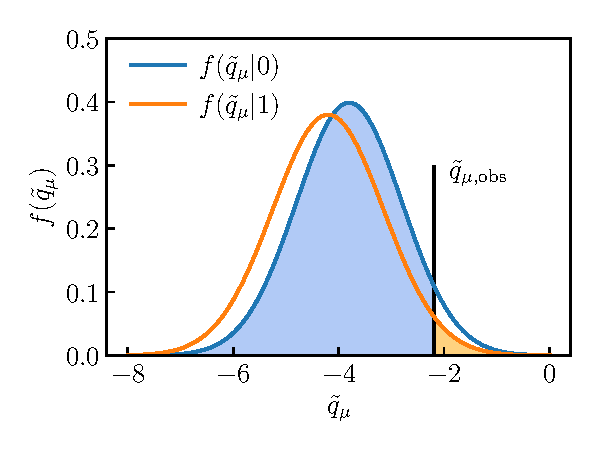
\includegraphics[width=\textwidth]{cls_1}
		\caption{\label{fig:cls_close}}
	\end{subfigure}%
	\begin{subfigure}[b]{0.45\linewidth}
		\centering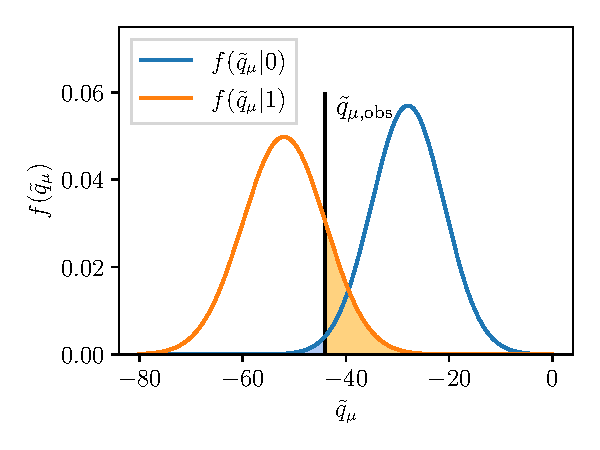
\includegraphics[width=\textwidth]{cls_2}
		\caption{\label{fig:cls_far}}
	\end{subfigure}%
	\caption{Distribution of the \glspl{pdf} of the signal plus background (in orange) and background-only (in blue) models. The coloured areas represent the $p_{s+b}$ and $p_{b}$ values, respectively. Figure~\subref{fig:cls_close} shows a case where both \glspl{pdf} are close together, while figure \subref{fig:cls_close} shows a case where both a well separated. Adapted from \cite{Cowan:2013pha}.}\label{fig:cls_method}
\end{figure}

In the $CL_{s+b}$ method, a signal plus background model is excluded if $p_{s+b} < \alpha$, where $\alpha$ is defined by the desired confidence level, typically $CL = 1 - \alpha = 95\%$, and $p_{s+b}$ can be calculated using the test statistic $\tilde{q}_\mu$ (with $\mu = 1$) introduced before. If the experiment has very low sensitivity to a specific signal plus background model, \eg because the production cross section is too low, the test statistic of the signal plus background model will be very close to that of the background-only model. In case of an underfluctuation in data, the $\mu = 1$ model can then falsely be excluded, even though no sensitivity is expected. \Cref{fig:cls_method} illustrates this with a simple example. In fact, the exclusion of models to which the experiment has no sensitivity has a probability of at least $\alpha$~\cite{Cowan:2013pha}.

This problem can be remedied by adopting the $CL_s$ method~\cite{Read:2002hq}, altering the threshold for excluding a model in a way to avoid exclusion of models to which the experiment has very low sensitivity. The $CL_s$ value is defined as
\begin{equation}
	CL_s = \frac{p_{s+b}}{1-p_b},
\end{equation}
where $p_b$ is the $p$-value of the background-only hypothesis. If the distributions of the test statistics for the signal plus background and the background-only models are close a small value of $p_{s+b}$ due to an underfluctuation in data will entail a large value of $p_b$. Consequently, in the calculation of the $CL_s$ value, $p_{s+b}$ will be penalised by $1-p_b$ (that will be close to 0), resulting in $CL_s > p_{s+b}$, preventing the exclusion of the signal plus background model. Conversely, in the case where the two test statistics are well-separated and $p_{s+b} < \alpha$, then $p_b$ will also be small and thus $CL_s$ will be close to $p_{s+b}$ obtained by the frequentist approach. 



\section{Sensitivity estimation}\label{sec:sensitivity_estimation}


When designing search regions for an analysis, it is necessary to achieve an optimal signal-to-background separation power. A significance metric is needed in order to quantify the separation power and have a metric to optimise for. In the following, the expected discovery significance introduced in \reference\cite{Cousins:2007bmb} is used. As the full statistical model is in general not yet known when designing the search regions, appropriate assumptions have to be made. In a \textit{cut-and-count} selection where only the total number of events after a selection are relevant (and not \eg their distribution), the significance is determined by the total number of signal events $S$, the total number of background events $B$ and the uncertainty on the expected number of background events $\Delta B$. This can be modelled as a so-called \textit{on/off problem}~\cite{Cousins:2007bmb, CRANMER_2006}, where the cut-and-count experiment uses two bins, a \gls{sr} enriched in signal events, and a \gls{cr} containing only background events. The parameter $\tau = n_\mathrm{CR} / n_\mathrm{SR}$ then denotes the ratio between the event rate in the \gls{cr}, $n_\mathrm{CR}$, to the event rate in the \gls{sr}, $n_\mathrm{SR}$.

If $\tau$ is known, then the likelihood of this simple configuration can be written in terms of the expected background event rate
\begin{equation}
	L (\mu,B) = \mathrm{Pois}(n_{\mathrm{SR}}\vert\mu S + B) \cdot \mathrm{Pois}(nu_{\mathrm{CR}}\vert\tau B),
\end{equation} 
with $\mu$ the signal strength parameter. The relative background uncertainty can thus be treated as coming from a Poisson-distributed auxiliary measurement containing only background (\ie in the \gls{cr}) with corresponding uncertainty $\sqrt{\tau B}$, leading to the approximation
\begin{equation}
	\tau = \frac{B}{\Delta B^2}.
\end{equation}
As $n_{\mathrm{SR}}$ and $n_{\mathrm{CR}}$ are each drawn from a Poisson probability with unknown means $\nu_\mathrm{SR}$ and $\nu_\mathrm{CR}$, the background-only hypothesis corresponds exactly to the case where the ratio of Poisson means $\lambda = \nu_\mathrm{CR} / \nu_\mathrm{SR}$ is equal to $\tau$~\cite{Cousins:2007bmb}. The two Poisson terms can then be written as the product of a single Poisson term with mean $n_\mathrm{tot} = n_\mathrm{SR} + n_\mathrm{CR}$ and the binomial probability of picking $n_\mathrm{SR}$ events out of $n_\mathrm{tot}$ with probability $\rho = \nu_\mathrm{SR} / \nu_\mathrm{tot} = 1 / (1+\lambda)$, yielding for the likelihood
\begin{equation}
\begin{split}
	L(\mu, B) & = \mathrm{Pois} (n_\mathrm{tot}\vert\lambda_\mathrm{tot})\cdot B(n_\mathrm{SR}\vert\rho,n_\mathrm{tot}) \\ 
	& = \frac{e^{-\lambda_\mathrm{tot}}\lambda_{\mathrm{tot}}^{n_\mathrm{tot}}}{n_\mathrm{tot}\,!} \cdot{n_\mathrm{tot}\choose n_\mathrm{SR}} \rho^\lambda_\mathrm{tot} (1-\rho)^{n_\mathrm{tot}-n_\mathrm{SR}}.
\end{split}
\end{equation}

Since the background-only hypothesis can not only be expressed as $\mu = 0$, $\nu_\mathrm{SR} = \nu_B$, or $\lambda = \tau$, but especially also as $\rho = 1/(1+\tau)$~\cite{Cousins:2007bmb}, its $p$-value can be calculated using the well-know frequentist binomial test,
\begin{equation}
	p_\mathrm{B} = \sum_{j=n_\mathrm{SR}}^{n_\mathrm{tot}} B (j\vert n_\mathrm{tot}, \rho).
\end{equation}
The significance corresponding to $p_\mathrm{B}$ can be derived using~\cref{eq:significance} is computable in a numerically fast way using the incomplete beta function. The algorithm used for calculating $Z_\mathrm{B}$ in this work is implemented in the \texttt{RooStats::NumberCountingUtils} methods in \textsc{ROOT}.



